\documentclass[11pt]{article}

% Font
% \renewcommand{\familydefault}{\sfdefault}
% \usepackage{helvet}
% \usepackage[sfdefault,light]{roboto}

\usepackage[T1]{fontenc} %
% \usepackage[latin1]{inputenc} %
\usepackage[utf8]{inputenc} %
% \usepackage[applemac]{inputenc} %
% \usepackage{a4wide} %

% \setlength{\parskip}{0.3\baselineskip}

\usepackage{amsmath, amssymb, amsfonts, stmaryrd}
\usepackage{mathrsfs}
\usepackage{amsthm}
\usepackage{bm}
\usepackage{pifont}

% Add some colors
\usepackage[usenames,dvipsnames,svgnames,table]{xcolor}
\usepackage{hyperref}
\hypersetup{
 linktocpage,
 colorlinks,
 citecolor=BlueViolet,
 filecolor=red,
 linkcolor=Blue,
 urlcolor=BrickRed
}

% NTH
\usepackage[super]{nth}

% For EPS figures
\usepackage{graphicx}
\usepackage{epstopdf}
\usepackage{wrapfig}

% Theorems
\theoremstyle{plain}
\newtheorem{theorem}{Theorem}%[section]
\newtheorem{lemma}[theorem]{Lemma}
\newtheorem{corollary}[theorem]{Corollary}
\newtheorem*{note}{Note}
\newtheorem{definition}{Definition}

\theoremstyle{remark}
\newtheorem*{example}{Example}

% Meta comment
\newcommand\meta[1]{\noindent\textcolor{blue}{\emph{#1}}}

% Include the macro file
% evergreens
\newcommand{\der}{\,\vdash}
\newcommand{\Der}{\,\Vdash}

% semantic brackets
\def\lv{\mathopen{{[\kern-0.14em[}}}    % opening [[ value delimiter
\def\rv{\mathclose{{]\kern-0.14em]}}}   % closing ]] value delimiter
\newcommand{\den}[1]{\lv #1 \rv}
\newcommand{\Den}[3][]{\den{#2}^{#1}_{#3}}
\newcommand{\dent}[2]{\llparenthesis#1\rrparenthesis_{#2}}

% latin etc. abbrev
\newcommand{\abbrev}[1]{#1} % alternative: \emph{#1}
\newcommand{\cf}{\abbrev{cf.}\ }
\newcommand{\eg}{\abbrev{e.\,g.}}
\newcommand{\Eg}{\abbrev{E.\,g.}}
\newcommand{\ie}{\abbrev{i.\,e.}}
\newcommand{\Ie}{\abbrev{I.\,e.}}
\newcommand{\etal}{\abbrev{et.\,al.}}
\newcommand{\wwlog}{w.\,l.\,o.\,g.} % \wlog is ``write into log file''
\newcommand{\Wlog}{W.\,l.\,o.\,g.}
\newcommand{\wrt}{w.\,r.\,t.}

% Inference rules
\newcommand{\rulename}[1]{\ensuremath{\mbox{\sc#1}}}
\newcommand{\ru}[2]{\dfrac{\begin{array}[b]{@{}c@{}} #1 \end{array}}{#2}}
\newcommand{\rux}[3]{\ru{#1}{#2}~#3}
\newcommand{\nru}[3]{#1\ \ru{#2}{#3}}
\newcommand{\nrux}[4]{#1\ \ru{#2}{#3}\ #4}
\newcommand{\dstack}[2]{\begin{array}[b]{c}#1\\#2\end{array}}
\newcommand{\dru}[3]{\ru{\dstack{#1}{#2}}{#3}}
\newcommand{\tru}[4]{\dru{\dstack{#1}{#2}}{#3}{#4}}
\newcommand{\trux}[5]{\dru{\dstack{#1}{#2}}{#3}{#4}\ #5}
\newcommand{\qru}[5]{\tru{\dstack{#1}{#2}}{#3}{#4}{#5}}
\newcommand{\ndru}[4]{#1\ \ru{\dstack{#2}{#3}}{#4}}
\newcommand{\ndrux}[5]{#1\ \ru{\dstack{#2}{#3}}{#4}\ #5}

% Symbols and names
\newcommand\Type{\operatorname{Type}}
\newcommand\isnType[2]{\operatorname{is-}#1\operatorname{-Type}\ #2}
\newcommand\nType[1]{#1\operatorname{-Type}}
\newcommand\R{\operatorname{R}}
\newcommand\emb[2]{\operatorname{embedding}#1\ #2}
\newcommand\RRe[2]{\operatorname{RR_e}#1\ #2}
% \newcommand\type{\ \bm{\operatorname{type}}}
\DeclareMathOperator{\type}{\ \mathbf{type}}
\DeclareMathOperator{\ctr}{\mathbf{ctr}}
\DeclareMathOperator{\refl}{\mathbf{refl}}
\newcommand\rew{\searrow}
\newcommand\gettype{\operatorname{.type}}
\newcommand\getproof{\operatorname{.proof}}
\newcommand\Var{\operatorname{Var}}
\newcommand\Exp{\operatorname{Exp}}
\newcommand\Ctx{\operatorname{Ctx}}
\newcommand\Whnf{\operatorname{Whnf}}
\newcommand\Wne{\operatorname{Wne}}


\begin{document}

\title{Justifying Resizing Rules in HoTT \\
\small{Through an interpretation of extensional type theory into an intensional
one}}

\author{Théo Winterhalter, Nicolas Tabareau (ASCOLA, LINA)}

\date{\nth{5} of September, 2016}

\maketitle

\pagestyle{empty} %
\thispagestyle{empty}

%% Attention: pas plus d'un recto-verso!
% Ne conservez pas les questions


\subsection*{The general context}
% What is it about ? Where does it come from ?
% What is the state of the art in this area ?
Homotopy Type Theory (HoTT for short) is a new domain that aims to offer a new
axiomatisation of mathematics that allows to consider objects up to isomorphisms
(as a result of the univalence axiom which allows to derive an equality between
isomorphic types).
The underlying theory thus develops a lot of notions related to equality and its
treatment, in particular it theorises about equalities between equalities that
are often considered to be trivial as they are in Set Theory.

\subsection*{The research problem}

% What is the question that you studied ?
% Why is it important, what are the applications/consequences ?
% Is it a new problem ?
% If so, why are you the first researcher in the universe who consider it ?
% If not, why did you think that you could bring an original contribution ?
In type theory, and thus in proof assistants such as Coq or Agda, in order to
avoid paradoxes \emph{à la} Russel, we have to establish a hierarchy of
universes (the types of types). Without it, it would be possible to prove
\emph{false} in Coq for instance.
Nevertheless, the typing rules dealing with universes are purely syntactical
and can be seen as rough approximations to preserve consistency.
They can be annoying for the user and we can legitimately wonder whether we
can alleviate theses restrictions in some specific cases.

Stated by Vladimir Voevodsky, the \emph{resizing rules} allow to lower the
universe level of a type under special conditions. The way he presented them
would make type checking undecidable.
We studied the possibility of a definition better suited to implementation
as well as a justification that the rules we propose preserve the consistency
of the system.

\subsection*{Your contribution}

% What is your solution to the question described in the last paragraph ?
% Be careful, do \emph{not} give technical details, only rough ideas !
% Pay a special attention to the description  of the \emph{scientific} approach.
We propose a way to implement resizing rules in Coq (which will be possible in
the next release) with precise typing rules.
We then show that -- up to some axioms that are consistent in a univalent
setting -- all resizing rules that we proposed %(and that correspond to the ones
% of Voevodsky)
can be reduced to only one.
We finally show the consistency of this one rule by generalizing a result by
Nicolas Oury stating that we can translate extensional type theory into
intensional type theory in a univalent setting (up to now it relied on the
uniqueness of identity proofs that is incompatible with univalence).
This last step is, in itself, an interesting result.

\subsection*{Arguments supporting its validity}

% What is the evidence that your solution is a good solution ?
% Experiments ? Proofs ?
Our work consists of a proof and an implementation.
However, our proof relies on some axioms that we deem consistent in a univalent
setting but this would require more work to justify their use more explicitely.

% Comment the robustness of your solution:
% how does it rely/depend on the working assumptions ?

\subsection*{Summary and future work}

% What is next ? In which respect is your approach general ?
% What did your contribution bring to the area ?
% What should be done now ?
% What is the good \emph{next} question ?
Our approach goes through a very gereral interpretation of extensional type
theory into intensional type theory which is an interesting result unavailable
in homotopy type theory. Besides we allow the use of resizing rules in actual
proofs in Coq.
Still, as we pointed out, we rely on an axiom and it would be interesting to
see if it holds in the simplicial model which is the mainstream model of
univalent homotopy type theory.

\subsection*{Notes}

Given that this report might serve as a basis for articles we decided to write
it in English.

\newpage
\pagestyle{plain} %

\section{Homotopy Type Theory}

We will start by briefly presenting type theory and then go to its homotopic
counterpart.

\subsection{Proof Theory and Proof Assistants}

The Curry-Howard isomorphism sets the basis for seeing $\lambda$-terms as
proofs and types as propositions. Since then, many systems such as
Martin-L\" of Type Theory (the theory behind Agda) or the Calculus of
Inductive Constructions (CIC -- the theory behind Coq) extended it to dependent
types that allow types to depend on terms.
% This way, the dependent product $\Pi x:A.B$ (where $B$ can mention $x$)
% represents the proposition $\forall x:A, B$.
We shall assume the reader is familiar with basic concepts associated to CIC
such as the inductive types as CIC will serve as our implicit context.

\subsection{Proofs and Equality}

Even though in Coq, one notion of equality is built-in, the conversion which
identifies terms up to $\beta$-reductions, it is often interesting to talk
about equality inside of proof terms.
We thus use the so-called identity types $\Id\ A\ u\ v$, meaning the type of
proofs that $u$ and $v$ of type $A$ are equal. It is often written
$u =_A v$ or even $u = v$ when $A$ is understood.
$\Id\ A\ x\ x$ have one inhabitant: $\refl_x$,
basically this means that we can only prove equality of objects that are already
convertible without relying on hypotheses of course: this is the smallest
reflexive relation.

\begin{wrapfigure}{r}{0.25\textwidth}
    \centering
    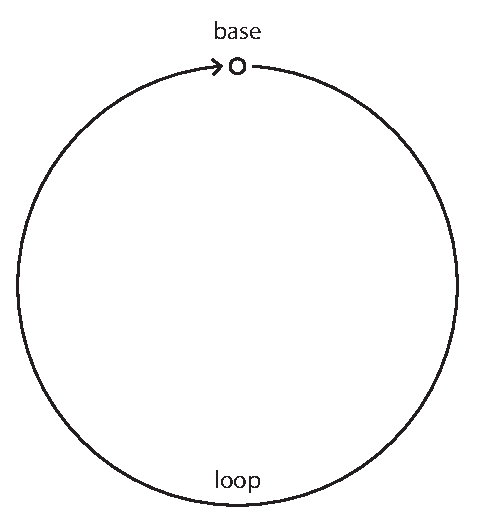
\includegraphics[scale=.4]{s1.eps}
\end{wrapfigure}
Homotopy type theory comes with concepts that tend to inhabit equlity through
other means than reflexivity. For instance, it introduces the notion of
\emph{higher inductive types} that are not only described by constructors but
also by equalities.
The most standard example is probably the circle $\S1$ that has one constructor
$\base : \S1$ and one non-trivial equality $\sloop : \base = \base$
(in the figure on the right we implicitely see an equality as a directed arrow).
This can go against the intuition but this type doesn't have only one element,
\ie it is not provable that $\forall x,y : \S1.\ x = y$. It is however
reassuring that the circle doesn't consist of only one point.
All equalities in $\sloop = \sloop$ aren't provably equal either.
However, for a type such as $\bool$ whose elements are not all
identifiable (we can even prove $\true \neq \false$), we can prove that all
proofs of $b =_{\bool} b$ are equal, but this does not come easily.
This gives rise to a classification of types depending on the properties
of their (higher) equalities.

\begin{definition}[$n-\Type$s]
  \leavevmode
  \begin{itemize}
    \item We say a type $T$ is \emph{contractible} (or a $(-2)-\Type$) when
          there is $t : T$ such that $\forall x : T. x = t$.
    \item We say that $T$ is an $(n+1)-\Type$ when for all $x, y : T$, the type
          $x =_T y$ is an $n-\Type$.
  \end{itemize}
\end{definition}
%
\noindent
In particular, we shall say that a $(-1)-\Type$ is a \emph{(mere) proposition}
following the intuition that such a type is either \emph{true} ($\top$ -- the
unit type) or \emph{false} ($\bot$ -- the empty type).
We also say that a $0-\Type$ is a \emph{set} as it verifies uniqueness of
identity proofs as sets of set theory.

For instance, $\bool$ is a set as all proofs of $b_1 = b_2$ are equal, but it
is not a mere proposition because $\true = \false$ is not inhabited and thus
not contractible.

\paradot{Transport}
We represented the circle by drawing $\sloop$ as a path from $\base$ to
$\base$, this way of representing the equality can be explicited by the notion
of transport.
Basically, given $p : A =_{\Type} B$, it is possible to construct a function
$p_* : A \to B$ using the elimination principle of equality.

\paradot{Operations}
The elimination principle for equality can be annoying to use in general so we
rather prove basic lemmata that make reasoning about equality easier.
One that is useful for instance is the congruence of equality under application:
\[ \ap : \forall (f : A \to B).\ x =_A y \to f\ x =_B f\ y. \]
\noindent
It has a precise definition that we won't state here, but it basically
follows directly from the elimination principle of the equality.

Similarly for any $p : x = y$ and $q : y = z$, we can define
$p\inv : y = x$ and $p \cons q : x = z$ translating symmetry and transitivity.

\subsection{Univalence}

As we already mentioned, univalence is a principle that basically allows to
identify objects that are equivalent. To really give meaning to those words we
need to define what we mean by equivalence.

\begin{definition}[Equivalence]
  Given $A$, $B$ and $f : A \to B$, we say that $f$ is an equivalence
  if there exist the following terms:
  \begin{itemize}
    \item $g : B \to A$,
    \item $\eta : \forall a:A.\ g\ (f\ a) = a$,
    \item $\epsilon : \forall b:B.\ f\ (g\ b) = b$,
    \item $\alpha : \forall a:A.\ \ap\ f\ (\eta\ a) = \epsilon\ (f\ a)$.
  \end{itemize}
  We write $A \approx B$ for the type of equivalences between $A$ and $B$.
\end{definition}

\noindent
An interesting to remark is that if $A$ and $B$ are sets, then an equivalence is
exactly a bijection between types (which incidently is the notion of isomorphism
for sets).

Using transports it is trivial to construct an equivalence between two equal
types $A = B$ which gives us an arrow $f : (A = B) \to (A \approx B)$.
The principle of univalence states that this arrow itself is an equivalence.

\begin{definition}[Univalence]
  The univalence axiom states that
  the trivial arrow $(A = B) \to (A \approx B)$ is itself an equivalence.
\end{definition}

\noindent
This means in particular that two equivalent types are equal (which is usually
how univalence is presented to people that aren't familiar with homotopy type
theory) but it actually says more. The way to construct the equality is related
to the equivalence.
For instance, if you take a look at $\bool$, there are two ways to prove
$\bool = \bool$, the usual straightforward way which corresponds to the identity
and the twisted way coming from univalence that exchanges $\true$ and $\false$.

\section{Resizing Rules}

We will now present the resizing rules and try to justify their need.

\subsection{Motivations}

Consistency in Coq relies on a hierarchy of universes $\Type_i$ with
$\Type_i : \Type_{i+1}$. Even though this is usually transparent to the user
(who only sees $\Type$), sometimes the user gets presented with a
``universe inconsistency''. This happens for instance when a function was
defined over $\Type_3$ but we provided a type in $\Type_4$.
This is of course the expected behavior, however in some cases the universe
level of an object grew artifically.

Take the notion of subsets: if we want to take a subset of $A$ satisfying
a given predicate $P$, we write $B := \{ x : A \mid P\ x \}$ in Coq.
The problem is that $P$ could live in high universes, making the universe level
of $B$ grow as well, meaning it could be bigger than the one of $A$ although
it was originally intended as a subset of $A$.
The consequences are that some properties of $A$ might not be inherited by
$B$ because of universe constraints.
One of the resizing rules proposed by Vladimir Voevodsky states that any
mere proposition can be taken in the smallest universe ($\Type_0$).
In our case it would lower the universe of $P\ x$ and $B$ would fit in the same
universe as $A$.

This is meant as a motivation to research resizing rules but this does not mean
that they are necessary or even strengthen our system.
We will consider them as a tool that makes your life better when dealing with
universe problems in Coq.

\subsection{Original Statement}

In a talk he gave, Vladimir Voevodsky proposed several resizing rules that would
be helpful in UniMath, a formalisation of univalent foundations of mathematics
in Coq. At the time of the writing, they are using the option ``type-in-type''
(which allows $\Type : \Type$, collapsing the universe hierarchy) to avoid
those universe problems.

The first one is the one we already mentioned that says that mere propositions
are small. It is consistent with the remark we made about mere propositions
saying that they are intuitively $\top$ or $\bot$ which incidentally live in
$\Type_0$. We write $\ishProp\ T$ the type of proofs that $T$ is a mere
proposition.

\begin{mathc}
  \ru{\Gamma \der h : \ishProp\ T
    }{\Gamma \der T : \Type_0}
\end{mathc}

$\hProp$, the type of mere propositions (a $\Sigma$-type containing a type $T$
and a proof $\ishProp\ T$), can be seen as $\bool$ if we extend our intuition
to saying that it only contains $\top$ and $\bot$. We also would like to put in
the smallest universe.

\begin{mathc}
  \ru{}{\Gamma \der \hProp : \Type_0}
\end{mathc}

If we consider two types to be equal, it only seems natural that they can live
in the same universe. As of now, if $A : \Type_i$ and $B : \Type_j$, then we
can consider $A =_{\Type_{\max(i,j)}} B$ in the biggest universe of the two
when we would like to see both of them in the smallest.
This gives the following rule:

\begin{mathc}
  \ru{A : \Type_i \qquad
      e : A = B
    }{B : \Type_i}
\end{mathc}

Similarly (especially if we think in univalent terms), we can state a rule for
equivalence that generalize the previous one:

\begin{mathc}
  \ru{A : \Type_i \qquad
      h : A \approx B
    }{B : \Type_i}
\end{mathc}

As one can see, these rule seem to break decidability of type checking, hence
the need for a more explicit statement of those rules.

\subsection{Implementation Proposal}

In order to preserve decidability of type checking, we explicit tag the resized
version of a type by $\RR$. For instance, the rule for equivalence becomes:

\begin{mathc}
  \ru{A : \Type_i \qquad
      B : \Type_j \qquad
      h : A \approx B
    }{\RR\ A\ h : \Type_j}
\end{mathc}

\noindent
However, we need to relate $\RR\ A$ (we will ignore the $h$ as it is understood
in most cases) and $A$ in some way. Mike Shulman for instance proposed to say
that $\RR\ A$ and $A$ are equivalent, but in this precise case, this is not
really interesting as we could have used $B$ from the start.
Instead we use a \emph{strict equivalence}:

\begin{mathc}
  \ru{\Gamma \der t : A
    }{\Gamma \der \inj\ t : \RR\ A}
  \qquad
  \ru{\Gamma \der t : \RR\ A
    }{\Gamma \der \proj\ t : A}
\end{mathc}
%
\noindent
such that $\proj\ (\inj\ t) \equiv t$ and $\inj\ (\proj\ t) \equiv t$ are
conversions that hold in the system (the equalities of the equivalence are not
only provable but definitional).
This corresponds to records with primitive projections in Coq, hence the
decidability.
%
This can be achived in Coq thanks to Pierre-Marie Pédrot by deactivating the
universe checking locally to create a records that holds a value of type $A$.

All the rules can be treated similarly.

\meta{Mention the surjection rule somehow?}


\section{One Rule to Resize Them All}

As a means to justify the consistency of those rules, we wondered if was not
possible to reduce all rules to one. We show here several candidates.

\subsection{Embedding}
The fist candidate we had was the embedding resizing rule.
We say that $f : A \to B$  is an \emph{embedding} when $\ap\ f$ is an
equivalence (we write $A \embd B$ for the type of embeddings).
To put it simply, we have $(x =_A y) \approx (f\ x =_B f\ y)$.
For sets, it corresponds to injective maps:
$f\ x = f\ y \to x = y$.
In such a case it feels natural to consider $A$ to be smaller than $B$:

\begin{mathc}
  \ru{\Gamma \der A : \Type_i \qquad
      \Gamma \der B : \Type_j \qquad
      \Gamma \der h : A \embd B
    }{\Gamma \der \RR\ A : \Type_j}
\end{mathc}

\noindent
This was a good candidate in the sense that any mere proposition can be embedded
in $\top$ and that $A \approx B$ implies $A \embd B$.
However, this does not allow us to resize $\hProp$ itself and we were not able
to find a good justification for it.

\subsection{Equivalence}
If we are ready to rely on some axioms we can reduce all the resizing rules we
mentioned (even the embedding one) to the equivalence resizing rule.
For instance, the equality can trivially be reduced to equivalence.
The other need more work and we shall detail them below.

\paradot{Mere Propositions}
In HoTT with univalence, the excluded-middle $\forall T.\ T + \neg T$ is
inconsistent. However its restriction to mere propositions can be safely
assumed.
\[\emd : \forall (T:\hProp).\ T + \neg T.\]
In a way, it makes sense as we really want to decide wheter a proposition is
true or not rather than whether a type is inhabited or not.

Once we have that, for any mere proposition $T$, we can create the type $T'$
that is $\top$ or $\bot$ depending on the result of $\emd\ T$.
That way $T' : \Type_0$ and $T \approx T'$.
We can conclude it is safe to assume the resizing of mere propositions as long
as it is safe to assume the excluded-middle for them and the resizing of
equivalence.

Likewise, we can show that $\hProp \approx \bool$ using $\emd$ in the same
fashion, and, since $\bool : \Type_0$, the resizing rule of $\hProp$ is also
reducible to equivalence.
\meta{Doesn't it use univalence as well?}

\paradot{Embeddings}
\meta{Say it is equivalent to the image of $f$, how much into details should we
go? As for the rest, we should probably have it proven in a Coq file and leave
it to the interested reader.}

\subsection{Equality}
It is tempting to say that equivalence is the one rule that generalizes all the
others, however for the purpose of the proof, it is worth noting that under
univalence we can reduce it to the equality rule.
Once we have $e : A = B$ it feels like we could simply choose $\RR\ A$ to be
$B$ and use $e$ and $e\inv$ respectively for $\inj$ and $\proj$,
however, unless $e = \refl$, $e\inv_*\ (e_*\ t) \equiv t$ does not hold
definitionally.

Nevertheless, if we could turn $A = B$ into $A \equiv B$, we would have won.

\section{Extensional to Intensional}

\subsection{State of the Art}

In order to justify the resizing rule for equality, we would like to transform
a propositional equality into a conversion rule:

\begin{mathc}
  \ru{\Gamma \der p : u = v
    }{\Gamma \der u \equiv v}
\end{mathc}
%
The above rule is a bridge between intensional and extensional type theory.
Extensional type theory is more powerful as the equality is able to relate a lot
more terms. This comes at the price of decidability for the type checking but it
is still used in proof assistants like Nuprl or Andromeda.

Nicolas Oury proposed a proof of the consistency of such an extension of coq by
creating a program translation that associates a derivation in the extensional
calculus to a derivation in the intensional one such that a proof of $\bot$
is translated to a proof of $\bot$.
The problem is that this translation relies on the uniqueness of identity
proofs (UIP) that is not compatible with univalence.

It is worth noting that Van Doorn \etal proposed a similar proof by showing the
equivalence between a PTS (Pure Type System) with explicit conversion and one
without. Indeed, the translation from the extensional type theory maps
conversions to transports that can be seen as explicit conversions.

\subsection{Translation compatible with Univalence}

As we said, the work of Nicolas Oury relies on UIP -- which cannot be assumed in
HoTT -- but in name only. Indeed, if we only assume it for equalities over
type, namely:
\[ \forall (p : \Type_i = \Type_i).\ p = \refl, \]
then we can adapt the proof so that it still holds.
There is of course the question of whether it is safe to assume it and, while
we don't have a definite proof, it appears that for parametricity reasons,
it is not possible to build an equivalence between $\Type_i$ and itself that
is not the identity.

Let us now detail the adapted proof.

\subsubsection{(Extensional) Calculus of Constructions}

Our goal is to translate judgements in the Extensional Calculus of
Constructions (herafter called \CCe) into the regular Calculus of Constructons
(CC). Contexts will be either the empty context $\cdot$ or of the form
$\Gamma, x:T$ and $\der \Gamma$ shall mean that the context $\Gamma$ is
well-formed.

We will write $s$ for sort variables, sorts being of the form $\Type_i$ for
some $i$. CC is also equipped with a relation between sorts for the function
spaces formation: $(\Type_i, \Type_j, \Type_{\max(i,j)})$.

The typing rules of CC are given in figure~\ref{fig:cc-typ} while its
convertibility rules (judgements of the form $\Gamma \der t \equiv t'$) are
given in figure~\ref{fig:cc-conv}.

\begin{figure}[h]
  \hrule \vspace*{2ex}%

  \begin{mathc}
    \nmru{ECon}{}{\der \cdot}
    \qquad
    \nmru{I-Con%
        }{\Gamma \der A : s
        }{\der \Gamma, x:A}
    \qquad
    \nmrux{Var%
         }{\der \Gamma
         }{\Gamma \der x : A
         }{(x : A) \in \Gamma}
  \end{mathc}

  \begin{mathc}
    \nmru{Type}{}{\Type_i : \Type_{i+1}}
    \qquad
    \nmru{Univ%
        }{\Gamma \der A : \Type_i
        }{\Gamma \der A : \Type_{i+1}}
  \end{mathc}

  \begin{mathc}
    \nmrux{Prod%
         }{\Gamma \der A : s_1 \qquad
           \Gamma, x:A \der B : s_2
         }{\Gamma \der \forall x:A.B : s_3
         }{(s_1,s_2,s_3)}
  \end{mathc}

  \begin{mathc}
    \nmru{App%
        }{\Gamma \der t : \forall x:A.B \qquad
          \Gamma \der u : A
        }{\Gamma \der t\ u : B[x := u]}
    \qquad
    \nmru{Lam%
        }{\Gamma, x:A \der t : B
        }{\Gamma \der \lambda x:A.t : \forall x:A.B}
  \end{mathc}

  \begin{mathc}
    \nmru{Conv%
        }{\Gamma \der A \equiv B \qquad
          \Gamma \der t : A \qquad
          \Gamma \der B : s
        }{\Gamma \der t : B}
  \end{mathc}

  % \vspace*{2ex} \hrule%
  \hrule%

  \caption{Typing Rules of CC}
  \label{fig:cc-typ}
\end{figure}

\begin{figure}[h]
  \hrule \vspace*{2ex}%

  \begin{mathc}
    \nmru{$\beta$%
        }{\Gamma \der (\lambda x:A. t)\ u : T
        }{\Gamma \der (\lambda x:A. t)\ u \equiv t[x := u]}
    \qquad
    \nmru{CApp%
        }{\Gamma \der t_1 \equiv t_2 \qquad
          \Gamma \der u_1 \equiv u2
        }{\Gamma \der t_1\ u_1 \equiv t_2\ u_2}
  \end{mathc}

  \begin{mathc}
    \nmru{CProd%
        }{\Gamma \der A_1 \equiv A_2 \qquad
          \Gamma, x:A_1 \der B_1 \equiv B_2
        }{\Gamma \der \forall x:A_1.B_1 \equiv \forall x:A_2.B_2}
  \end{mathc}

  \begin{mathc}
    \nmru{CLam%
        }{\Gamma \der A_1 \equiv A_2 \qquad
          \Gamma, x:A_1 \der t_1 \equiv t_2
        }{\Gamma \der \lambda x:A_1.t_1 \equiv \lambda x:A_2.t_2}
  \end{mathc}

  \hrule%

  \caption{Convertibility Rules of CC}
  \label{fig:cc-conv}
\end{figure}

In order to obtain \CCe we only add the extensionality rule below.
All judgements in \CCe will be written with $\dere$ whereas CC will use $\der$.
\begin{mathc}
  \nmru{Ext%
      }{\Gamma \dere p : u_1 = u_2
      }{\Gamma \dere u_1 \equiv u_2}
\end{mathc}

Please remark that, as in the work by Nicolas Oury, we will not speak about the
typing rules of the propositional equality as it would hinder readability.
Besides, our translation will actually go in the Calculus of Inductive
Constructions, the theory of Coq at full power with inductive types,
pattern-matching and fixpoints. It will also be extended with a few axioms
that we will discuss later.

\subsubsection{Principle of the Translation}

\subsubsection{Heterogenous Equality}

\subsubsection{Main Difficulty}

\subsubsection{Term Equivalence}

\subsubsection{Proof of the Translation}

\section*{Conclusion}

\end{document}
